%%%%%%%%%%%%%%%%%%%%%%%%%%%%%%%%%%%%%%%%%%%%%%%%%%%%%%%%%%%%%%%%%%%%%%%%%%%%%%%
% Copyright 2020
% Little Compline with Akathist to the Theotokos
% as  served on the first 4 Fridays of Great Lent
%%%%%%%%%%%%%%%%%%%%%%%%%%%%%%%%%%%%%%%%%%%%%%%%%%%%%%%%%%%%%%%%%%%%%%%%%%%%%%%

\documentclass[twoside, letterpaper, 12pt]{report}
\usepackage{orthodoxservicebook}

\title{Little Compline with Akathist to the Theotokos\\
       As served on the first four Fridays of Great Lent}
\author{St. Katherine Orthodox Church}
\date{}% Remove date

\titlepic{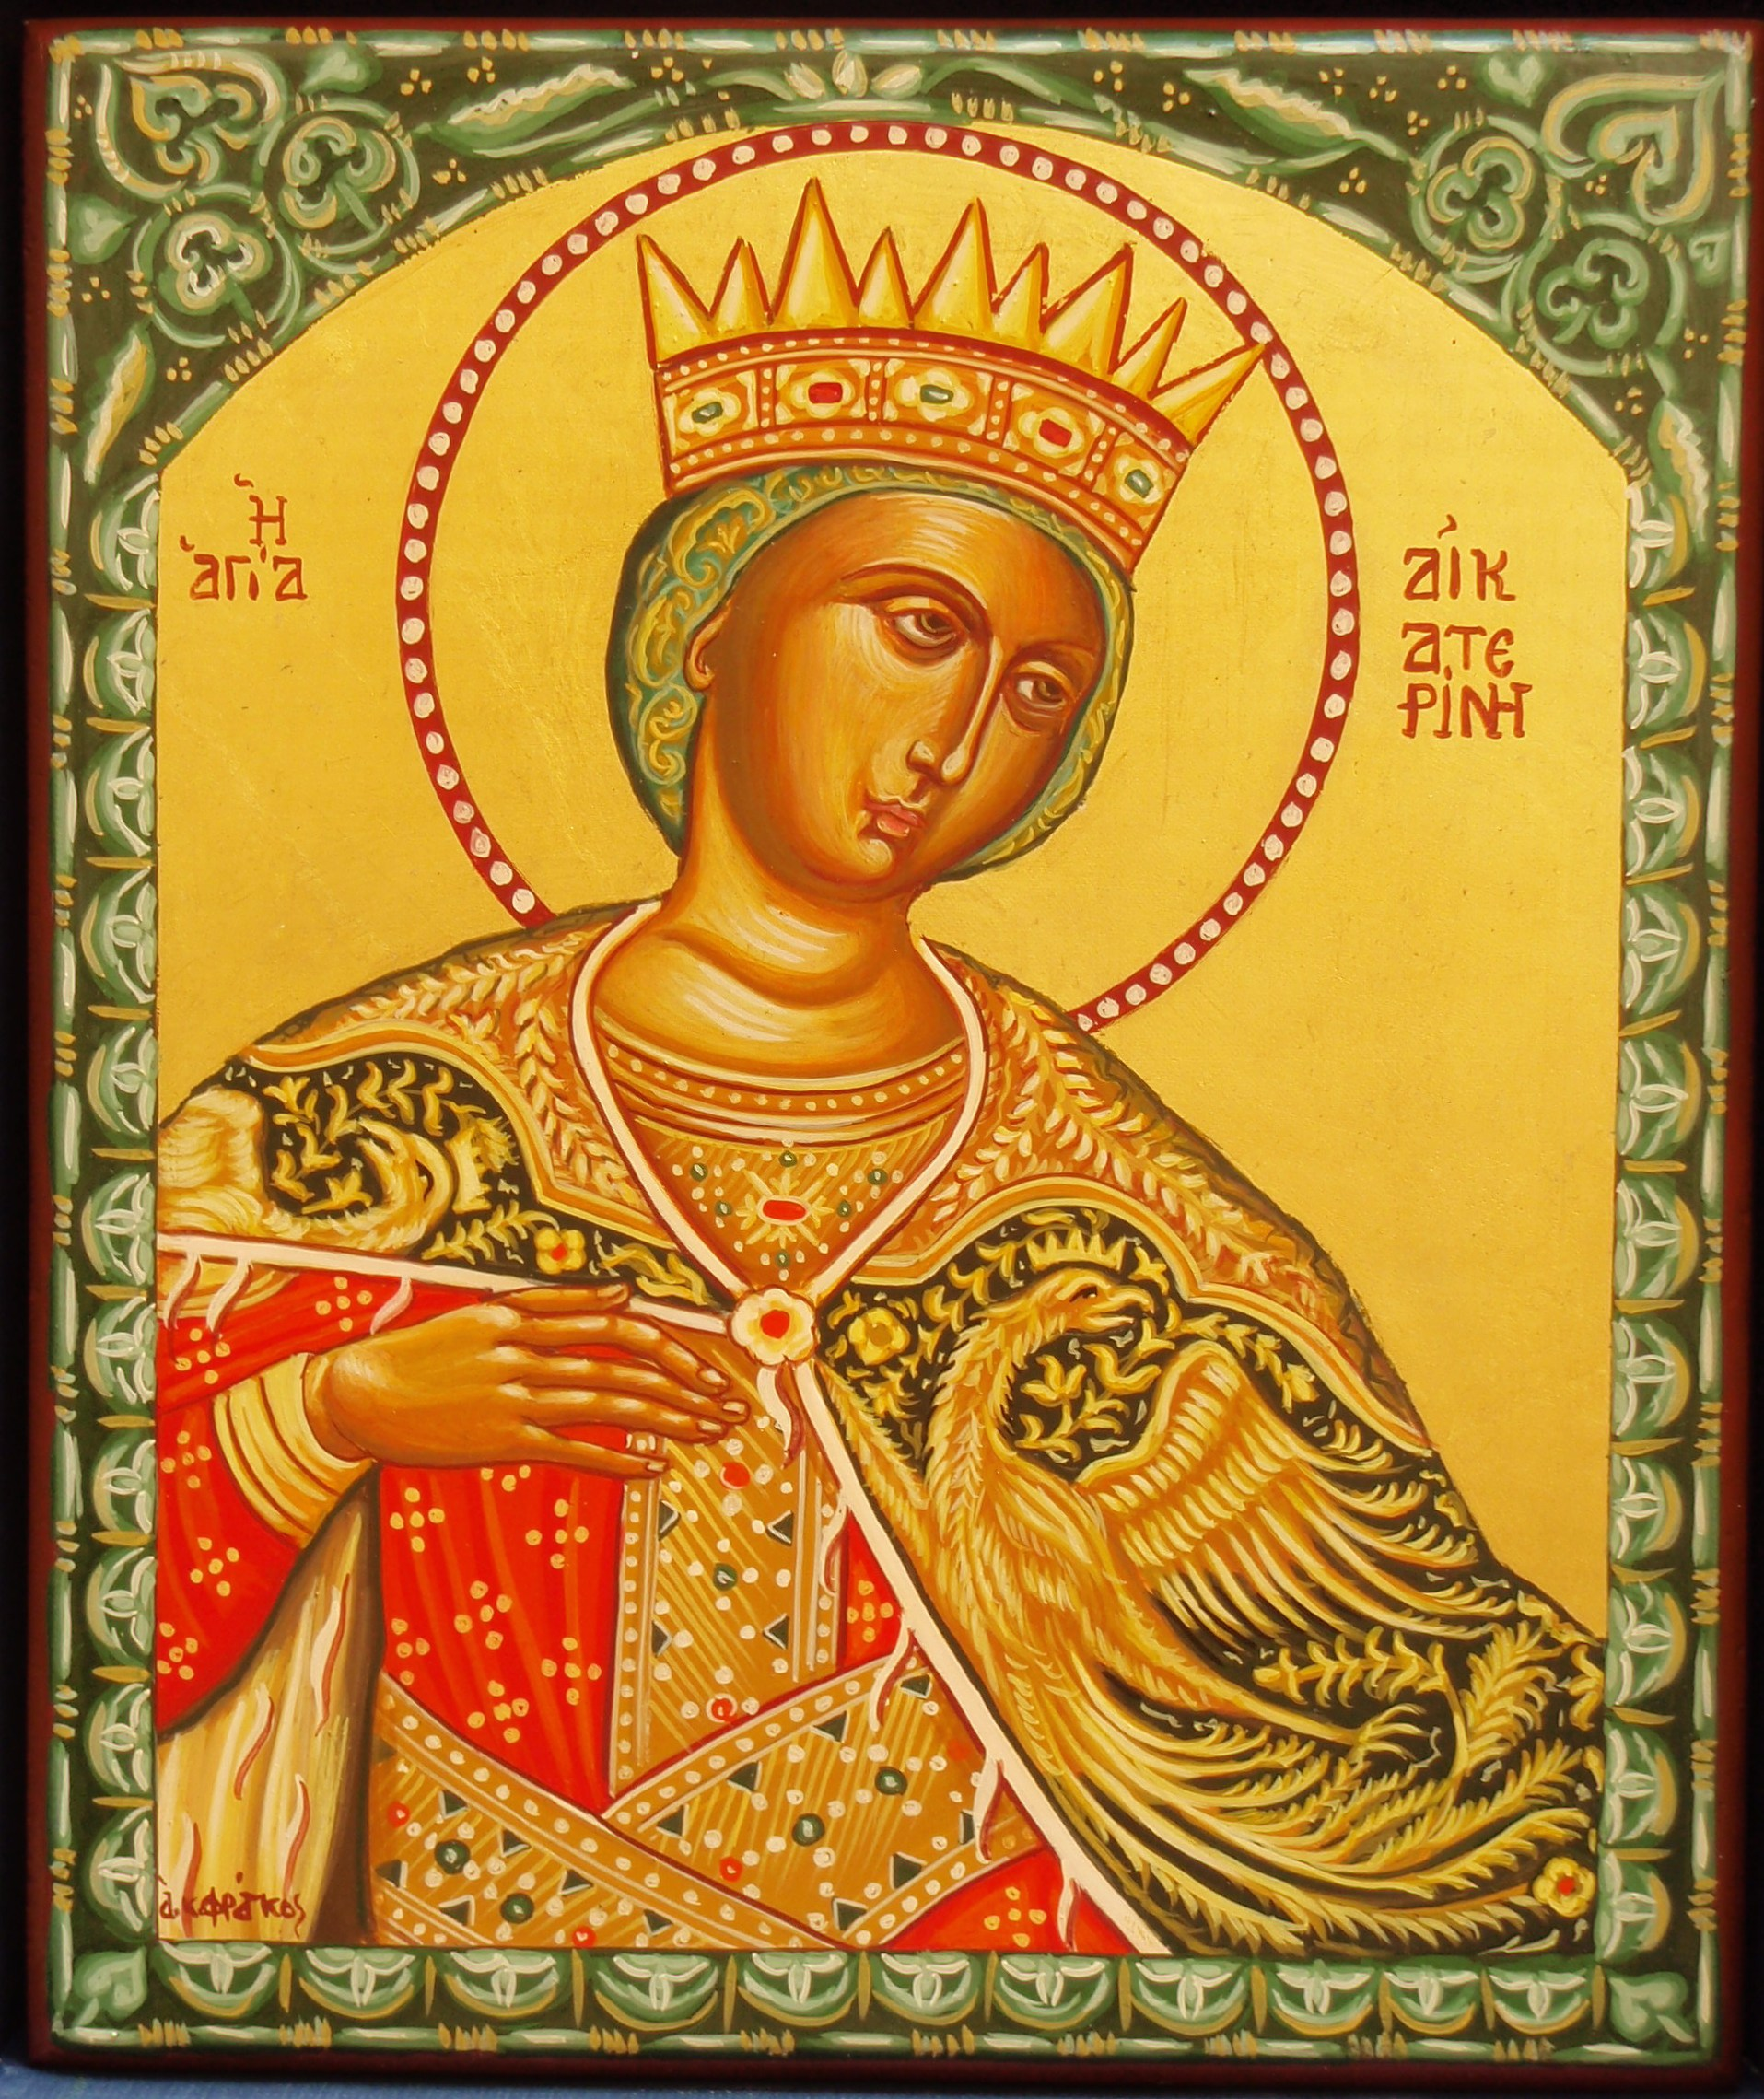
\includegraphics[width=0.5\textwidth]{Katherine1.jpg}}

\begin{document}
\maketitle
\pagestyle{empty} % Don't show page numbers

\instruction{This page intentionally left blank}

\cleardoublepage
\pagestyle{plain}
\setcounter{page}{1}

\chapter*{Little Compline, First Half}
\begin{priest}
\item Blessed is our God, always, now and ever, and unto ages of ages.
\end{priest}

\choralresponse{./Z-Responses/RussianPresanctified/Amen.ly}

\begin{priest}
\item Glory to Thee, our God. Glory to Thee.
\item O heavenly King, Comforter, the Spirit of truth,
who art everywhere present and fillest all things,
the Treasury of good things and Giver of life:
Come and abide in us and cleanse us from every stain and save our souls,
O Good One.
\end{priest}

\centeredsection{The Trisagion Prayers}
\instruction{Recited together as a congregation}

Holy God, Holy Mighty, Holy Immortal: have mercy on us. \instruction{(THRICE)}

\vbox{}
\emph{Glory to the Father, and to the Son, and to the Holy Spirit; both now and ever, and
unto ages of ages. Amen.}

\vbox{}
All-holy Trinity, have mercy on us. Lord, cleanse us from our sins. Master, pardon
our iniquities. Holy God, visit and heal our infirmities for Thy Name’s sake.

\vbox{}
Lord, have mercy. \instruction{(3x)}

\vbox{}
\emph{Glory to the Father, and to the Son, and to the Holy Spirit; both now and ever, and
unto ages of ages. Amen.}

\vbox{}
Our Father, Who art in Heaven, hallowed be Thy Name. Thy kingdom come; Thy
will be done on earth as it is in Heaven. Give us this day our daily bread; and forgive
us our trespasses, as we forgive those who trespass against us, and lead us not into
temptation, but deliver us from evil.

\begin{priest}
\item For Thine is the kingdom, and the power, and the glory:
    of the Father, and of the Son, and of the Holy Spirit; now and ever, and unto ages of ages.
\end{priest}

\choralresponse{./Z-Responses/RussianPresanctified/Amen.ly}

\begin{reader}
\item Lord, have mercy. \twelve
\item Glory to the Father, and to the Son, and to the Holy Spirit;
  both now and ever, 
  and unto ages of ages. Amen.

\item O come, let us worship and fall down before God our King.\\
  O come, let us worship and fall down before Christ, our King and our God.\\
  O come, let us worship and fall down before the Very Christ, our King and our God.
\end{reader}

\begin{maybetwocolumns}

\centeredsection{Psalm 50}
\input{Psalms/Psalm050.txt}

\centeredsection{Psalm 69}
\input{Psalms/Psalm069.txt}

\centeredsection{Psalm 142}
\input{Psalms/Psalm142.txt}

\centeredsection{The Little Doxology}
\instruction{Plain reading}
\begin{itemize}[label=\small{+},leftmargin=*]
\item Glory to God in the highest, and on earth peace, good will among men.
\item We praise Thee, we bless Thee, we worship Thee, we glorify Thee;
      we give thanks unto Thee for Thy great glory.
\item O Lord, heavenly King, God the Father Almighty;
      O Lord, the only-begotten Son, Jesus Christ; and the Holy Spirit.
\item O Lord God, Lamb of God, Son of the Father, Who takest away the sin of the world,
      have mercy on us; O Thou Who takest away the sins of the world.
\item Receive our prayer, O Thou Who sittest at the right hand of the Father,
      and have mercy on us.
\item For Thou only art holy, Thou only art the Lord, O Jesus Christ,
      to the Glory of God the Father. Amen.
\item Every day will I bless Thee, and I will praise Thy Name forever;
      yea, forever and ever.
\item Lord, Thou hast been our refuge in all generations.
      I said: Be merciful unto me; heal my soul, for I have sinned against Thee.
\item Lord, I have fled unto Thee: teach me to do Thy will, for Thou art my God.
\item For with Thee is the fountain of life: in Thy light shall we see light.
\item O continue Thy loving-kindness unto them that know Thee.
\item Vouchsafe, O Lord, to keep us this night without sin.
\item Blessed art Thou, O Lord God of our Fathers,
      and praised and glorified be Thy Name forever. Amen.
\item Let Thy mercy, O Lord: be upon us, as we do put our hope in Thee.
\item Blessed art Thou, O Lord: teach me Thy statutes.
\item Blessed art Thou, O Master; make me to understand Thy statutes.
\item Blessed art Thou, O Holy One; enlighten me with Thy statutes.
\item Thy mercy, O Lord, endureth forever.
      O despise not the works of Thy hands.
      To Thee belongeth worship, to Thee belongeth praise, to Thee belongeth glory:
      to the Father, and to the Son, and to the Holy Spirit;
      now and ever, and unto ages of ages. Amen.
\end{itemize}
\end{maybetwocolumns}

\centeredsection{The Nicene Creed}
\instruction{Recited together as a congregation}

\verbatiminput{Common/TheCreed.txt}

\squashedcenteredsection{Theotokon}
\instruction{Plain reading}

\readerline{\input{Common/ItIsTrulyMeetToBlessTheeOTheotokos.txt}}

\chapter*{The Canon of the Akathist}

\centeredsection{Ode One}
\lilypondfile{./4-Orthros/CanonOfTheAkathist-ToTheTheotokos/CanonOde1-Tone4-Kazan.ly}

\choralresponse{./Z-Responses/AkathistHymnBasil/MostHolyTheotokosSaveUs.ly}

When the great Archangel saw thee, O immaculate one,
thou living book of Christ, sealed by the Spirit, he cried unto thee:
Hail, vessel of gladness, through whom the curse of our first-mother is loosed.

\choralresponse{./Z-Responses/AkathistHymnBasil/MostHolyTheotokosSaveUs.ly}

Hail, virgin bride of God, thou uplifter of Adam and death-knell of Hades;
Hail, O all-blameless one, thou palace of the only King; Hail,
thou fiery throne of the Almighty.

\choralresponse{./Z-Responses/AkathistHymnBasil/GlorytoTheFSandHS.ly}

Hail, thou from whom alone didst blossom the Unwithering Rose;
Hail, thou who didst bear the fragrant Apple;
Hail, immaculate maiden, fragrance of the King of All and salvation of the world.

\choralresponse{./Z-Responses/AkathistHymnBasil/BothNowAndEver.ly}

Hail, thou treasure-house of purity, through which we rose up from our fall;
Hail, Lady, sweet-scented lily perfuming the faithful,
thou fragrant incense and most precious myrrh.


\centeredsection{Ode Three}

\lilypondfile{./4-Orthros/CanonOfTheAkathist-ToTheTheotokos/CanonOde3-Tone4-Kazan.ly}

\choralresponse{./Z-Responses/AkathistHymnBasil/MostHolyTheotokosSaveUs.ly}

As a clear and untilled field, thou didst make the Divine Ear of Grain to sprout;
Hail, thou living table that held the Bread of Life;
Hail, thou unfailing fountain of Living Water.

\choralresponse{./Z-Responses/AkathistHymnBasil/MostHolyTheotokosSaveUs.ly}

Hail, O mystic heifer that didst bear the Spotless Calf;
Hail, ewe-lamb who didst conceive the Lamb of God that taketh away the sins
of the whole world; Hail, thou fervent intercessor.

\choralresponse{./Z-Responses/AkathistHymnBasil/GlorytoTheFSandHS.ly}

Hail, O radiant dawn, which alone dost bear Christ the Sun, the dwelling-place of Light;
Hail, thou who didst dispel the darkness and reduce to naught the demons of gloom.

\choralresponse{./Z-Responses/AkathistHymnBasil/BothNowAndEver.ly}

Hail, thou only gate, through which the Word alone didst pass;
Hail, Lady, for by thy birth-giving the bars and gates of Hades were burst asunder;
Hail, thou most worthy of all praise, divine entry for the saved.


\centeredsection{Ode Four}

\lilypondfile{./4-Orthros/CanonOfTheAkathist-ToTheTheotokos/CanonOde4-Tone4-Kazan.ly}

\choralresponse{./Z-Responses/AkathistHymnBasil/MostHolyTheotokosSaveUs.ly}

In hymns of faith, O all-praised one, we cry out unto thee:
Hail, thou mountain fertile with the fullness of the Spirit;
Hail, thou lamp of light and vase of manna, to the senses of the reverent most sweet.

\choralresponse{./Z-Responses/AkathistHymnBasil/MostHolyTheotokosSaveUs.ly}

Hail, immaculate Lady, mercy-seat of the world;
Hail, thou ladder which raised all from earth to grace;
Hail, thou bridge which truly leads from death to life all who sing thy praises.

\choralresponse{./Z-Responses/AkathistHymnBasil/MostHolyTheotokosSaveUs.ly}

Hail, O immaculate one, higher than the heavens,
thou who didst without pain carry within thee the Foundation of the Earth.
Hail, O seashell that didst dip in thy blood the divine purple
for the King of the Powers of Heaven.

\choralresponse{./Z-Responses/AkathistHymnBasil/GlorytoTheFSandHS.ly}

Hail, Lady, who didst truly bear the Lawgiver
that freely blotted out the transgressions of all;
O unimaginable depth, O height ineffable, O maiden unwedded,
through whom we are become divine.

\choralresponse{./Z-Responses/AkathistHymnBasil/BothNowAndEver.ly}

With hymns we praise thee, O thou who didst weave for the world a crown not woven by hands;
Hail to thee, O Virgin, do we cry: fortress of all mankind,
and rampart, and strength, and refuge divine.


\centeredsection{Ode Five}

\lilypondfile{./4-Orthros/CanonOfTheAkathist-ToTheTheotokos/CanonOde5-Tone4-Kazan.ly}

\choralresponse{./Z-Responses/AkathistHymnBasil/MostHolyTheotokosSaveUs.ly}

Hail, O all-blameless one,
who didst bear the Way of Life and save the world from the deluge of sin;
Hail, bride of God, thou of great report and mighty fame;
Hail, thou dwelling-place of the Master of Creation.

\choralresponse{./Z-Responses/AkathistHymnBasil/MostHolyTheotokosSaveUs.ly}

Hail, O immaculate one, stronghold and fortress of mankind,
and place of hallowed glory, deathknell of Hades, bridal-chamber full of light;
Hail, joy of the angels;
Hail, help of those who faithfully pray unto thee.

\choralresponse{./Z-Responses/AkathistHymnBasil/MostHolyTheotokosSaveUs.ly}

Hail, O Lady, fiery chariot of the Word;
living paradise having the Lord, the Tree of Life, in thy midst;
His sweetness gives life to those who partake in faith,
even though they be subject to corruption.

\choralresponse{./Z-Responses/AkathistHymnBasil/GlorytoTheFSandHS.ly}

Strengthened by thy might, faithfully we cry unto thee:
Hail, city of the King of All, great in glory and repute,
of whom all these were clearly spoken;
O mount unhewn and depth beyond all measure.

\choralresponse{./Z-Responses/AkathistHymnBasil/BothNowAndEver.ly}

Thou spacious tabernacle of the Word,
Hail! O immaculate one, thou seashell which didst proffer the Divine Pearl;
Hail! O all-wondrous one, thou art the reconciliation to God,
O Theotokos, of all who ever bless thee.


\centeredsection{Ode Six}

\lilypondfile{./4-Orthros/CanonOfTheAkathist-ToTheTheotokos/CanonOde6-Tone4-Kazan.ly}

\choralresponse{./Z-Responses/AkathistHymnBasil/MostHolyTheotokosSaveUs.ly}

Immaculate bridal-chamber of the Word, and aid to the sanctification of us all,
Hail! O all-pure maiden, whom the Prophets did proclaim;
Hail, thou ornament of the Apostles!

\choralresponse{./Z-Responses/AkathistHymnBasil/MostHolyTheotokosSaveUs.ly}

From thee the dew distilled that quenched the flame of polytheism;
wherefore, we cry out unto thee, O Virgin:
Hail, O dewy fleece which Gideon did foresee.

\choralresponse{./Z-Responses/AkathistHymnBasil/GlorytoTheFSandHS.ly}

Behold, we cry out unto thee:
Hail! Be thou our haven and our port when we voyage
on the sea of tribulations and through the snares of the adversary

\choralresponse{./Z-Responses/AkathistHymnBasil/BothNowAndEver.ly}

O cause of joy, favor us with reason to cry out unto thee:
Hail, thou bush that burns yet unconsumed,
thou light-filled cloud which unceasingly shelters the faithful.


\centeredsection{Ode Seven}

\lilypondfile{./4-Orthros/CanonOfTheAkathist-ToTheTheotokos/CanonOde7-Tone4-Kazan.ly}

\choralresponse{./Z-Responses/AkathistHymnBasil/MostHolyTheotokosSaveUs.ly}

To thee we sing a hymn and cry: Hail! Chariot of the mystic sun,
true vine that did produce the ripe cluster of grapes,
dripping wine to gladden the souls of those who with faith do glorify thee.

\choralresponse{./Z-Responses/AkathistHymnBasil/MostHolyTheotokosSaveUs.ly}

Hail, thou Bride of God, who didst bear the Healer of Mankind;
the mystic staff from which blossomed the Unfading Flower;
Hail, O sovereign Lady, through whom we are filled with joy,
and made inheritors of life.

\choralresponse{./Z-Responses/AkathistHymnBasil/MostHolyTheotokosSaveUs.ly}

The tongue of eloquence has not power to sing thy praises,
O sovereign Lady, for thou wast exalted above the Seraphim
when thou didst bear Christ the King;
do thou now implore Him to deliver from all harm
those who faithfully reverence thee.

\choralresponse{./Z-Responses/AkathistHymnBasil/GlorytoTheFSandHS.ly}

The ends of the earth do praise and bless thee, and cry out unto thee:
Hail, pure Maiden, scroll on which the finger of God did inscribe His Word;
do thou now implore Him, O Theotokos,
to write down thy servants in the Book of Life.

\choralresponse{./Z-Responses/AkathistHymnBasil/BothNowAndEver.ly}

We thy servants bend the knee of our hearts and implore thee, O pure Maiden:
incline thine ear and save us, who are engulfed in tribulations;
and guard thy city, O Theotokos, from every assault of her enemies.

\centeredsection{Ode Eight}

\lilypondfile{./4-Orthros/CanonOfTheAkathist-ToTheTheotokos/CanonOde8-Tone4-Kazan.ly}

\choralresponse{./Z-Responses/AkathistHymnBasil/MostHolyTheotokosSaveUs.ly}

Thou didst receive the Word within thee, O pure Maiden,
and didst bear Him Who beareth all things;
thou didst nourish Him with milk, Who by His nod dost sustain all the universe;
to Him we sing: All ye works, praise the Lord, and magnify Him unto all ages.

\choralresponse{./Z-Responses/AkathistHymnBasil/MostHolyTheotokosSaveUs.ly}

Moses perceived in the burning bush the great mystery of thy birth-giving,
O chaste and holy Virgin;
the children prefigured this most clearly
when they stood in the midst of the flame and were un-burned;
wherefore, we praise thee unto all ages.

\choralresponse{./Z-Responses/AkathistHymnBasil/MostHolyTheotokosSaveUs.ly}

We, who of old were made naked by deceit,
have been clothed in a garment of incorruption by thy conception;
and we who were sitting in the darkness of transgressions
have come to see the light,
O Maiden who art the dwelling-place of Light:
wherefore, we praise thee unto all ages.

\choralresponse{./Z-Responses/AkathistHymnBasil/GlorytoTheFSandHS.ly}

Through thee the dead are made to live, for thou didst bear the Life Essential;
those who before were speechless now find useful eloquence,
lepers are cleansed, diseases are driven away,
and the multitude of aerial spirits are vanquished,
O Virgin, salvation of mortals.

\choralresponse{./Z-Responses/AkathistHymnBasil/BothNowAndEver.ly}

We hail thee, O all-blessed one,
who didst bring forth salvation for the world,
through which we have been raised from earth to heights above;
O pure Maiden, thou art shelter and stronghold,
bulwark and fortress of all who sing:
All ye works, praise the Lord, and magnify Him unto all ages.


\centeredsection{Ode Nine}

\lilypondfile{./4-Orthros/CanonOfTheAkathist-ToTheTheotokos/CanonOde9-Tone4-Kazan.ly}

\choralresponse{./Z-Responses/AkathistHymnBasil/MostHolyTheotokosSaveUs.ly}

Through thee, O Maiden, have we faithful become partakers of joy,
so that we may further cry out unto thee:
Hail! Do thou deliver us from perpetual temptation, from barbaric attack,
and from all the multitude of evils which we mortals suffer
for the number of our sins.

\choralresponse{./Z-Responses/AkathistHymnBasil/MostHolyTheotokosSaveUs.ly}

Thou hast appeared to enlighten us and be our confirmation,
wherefore we cry aloud to thee:
Hail, O unsetting star which didst introduce into the world the mighty Sun;
Hail, pure maiden, who didst open up fast-closed Eden;
Hail, fiery pillar, which doth lead man’s nature to the life above.

\choralresponse{./Z-Responses/AkathistHymnBasil/MostHolyTheotokosSaveUs.ly}

Let us stand with reverence in the house of our God, and let us cry aloud:
Hail, mistress of the world;
Hail, Mary, Lady of us all;
Hail, thou who alone art blameless among women, and beautiful;
Hail, O vessel, which didst receive into thyself the myrrh
which was never before outpoured.

\choralresponse{./Z-Responses/AkathistHymnBasil/GlorytoTheFSandHS.ly}

Hail, O Ever-virgin, thou dove who didst bring forth Him Who is merciful.
Hail, boast of all the righteous saints and crown of those who strive.
Hail, ornament divine of all the just, and of us the faithful,
our salvation as well.

\choralresponse{./Z-Responses/AkathistHymnBasil/BothNowAndEver.ly}

Spare, O God, Thine inheritance, and overlook now all our sins.
For as intercessor in Thy sight, O Christ,
there stands before Thee she that on earth conceived Thee without seed,
when in Thy Great Mercy
Thou hast willed to be shaped in a form that was not Thine own.

\centeredsection{Kontakion for the Akathist Hymn in Tone Eight}
\lilypondfile{./Menaion/03-25-AnnunciationOfTheTheotokos/AnnunciationOfTheTheotokos-Kontakion-T8-Essey-Music.ly}

%%%%%%%%%%%%%%%%%%%%%%%%%%%%%%%%%%%%%%%%%%%%%%%%%%%%%%%%%%%%%%%%%%%%%%%%%%%%%%%
%%%%%%%%%%%%%%%%%%%%%%%%%%%%%%%%%%%%%%%%%%%%%%%%%%%%%%%%%%%%%%%%%%%%%%%%%%%%%%%
\chapter*{Oikoi}
%%%%%%%%%%%%%%%%%%%%%%%%%%%%%%%%%%%%%%%%%%%%%%%%%%%%%%%%%%%%%%%%%%%%%%%%%%%%%%%
%%%%%%%%%%%%%%%%%%%%%%%%%%%%%%%%%%%%%%%%%%%%%%%%%%%%%%%%%%%%%%%%%%%%%%%%%%%%%%%

%%%%%%%%%%%%%%%%%%%%%%%%%%%%%%%%%%%%%%%%%%%%%%%%%%%%%%%%%%%%%%%%%%%%%%%%%%%%%%%
\centeredsection{First Stasis - First Friday of Great Lent}
%%%%%%%%%%%%%%%%%%%%%%%%%%%%%%%%%%%%%%%%%%%%%%%%%%%%%%%%%%%%%%%%%%%%%%%%%%%%%%%

\centeredsubsection{1. Oikos}
\begin{priest}
  \item An angel chieftain was sent from heaven to say 
    “Hail!” unto the Theotokos. \thrice{}
  \item … And beholding Thee, O Lord, taking bodily form,
    he stood rapt in wonder,
    and with bodiless voice cried aloud to her in this wise:
\end{priest}

\begin{itemize}[label=\tiny{+},leftmargin=*]
\item Hail, thou, through whom joy shall shine forth;
      Hail, thou, through whom the curse shall be destroyed.
\item Hail, thou restoration of fallen Adam;
      Hail, thou, redemption of the tears of Eve.
\item Hail, thou height untrodden by human minds;
      Hail, thou depth hard to scan, even for angels’ eyes.
\item Hail, thou that art a kingly throne;
      Hail, thou that holdest the Upholder of all.
\item Hail, thou star that showed the Sun;
      Hail, womb of the Divine Incarnation.
\item Hail, thou through whom Creation is renewed;
      Hail, thou through whom the Creator becomes
a babe.
\item Hail, O Bride without bridegroom! \instruction{The priest censes the icon.}
\end{itemize}

\lilypondfile{./Triodion/HailOBride-ForTheOikoi-T8-Basil-Music.ly}

\centeredsubsection{2. Kontakion}

\priestline{Boldly spake the holy maiden unto Gabriel,
  conscious of her chastity:
  To my soul thy strange message seems hard to grasp;
  how speakest thou of a virgin conception, crying aloud:
  Alleluia! \instruction{The priest censes the icon.}}

\lilypondfile{./Triodion/HailOBride-Alleluia-T8-Basil-Music.ly}

\centeredsubsection{3. Oikos}

\priestline{Craving to know knowledge unknowable,
  the Virgin cried out unto him who ministered unto her:
  From a maiden body, how may a Son be born;
  tell thou me! To her he spake in fear, and thus only cried aloud:}

\begin{itemize}[label=\tiny{+},leftmargin=*]
\item Hail, thou initiate of the ineffable counsel;
      Hail, O faith of those who pray in silence.
\item Hail, thou beginning of the miracles of Christ;
      Hail, thou crown of His decrees.
\item Hail, heavenly ladder, by which God came down;
      Hail, bridge that leadest us from earth to Heaven.
\item Hail, thou much-talked of wonder of angels;
      Hail, thou much-lamented damager of demons.
\item Hail, thou who ineffably didst bear the Light;
      Hail, thou who told none how it was done.
\item Hail thou, who over-soarest the knowledge of the wise;
      Hail, thou who enlightenest the minds of the faithful.
\item Hail, O Bride without bridegroom! \instruction{The priest censes the icon.}
\end{itemize}

\lilypondfile{./Triodion/HailOBride-ForTheOikoi-T8-Basil-Music.ly}

\centeredsubsection{4. Kontakion}
\priestline{Divine power from on high then overshadowed the maiden,
  that she might conceive, and showed forth her fruitful womb as a fertile field
  to all who desire to reap salvation, as they sing:
  Alleluia! \instruction{The priest censes the icon.}}

\lilypondfile{./Triodion/HailOBride-Alleluia-T8-Basil-Music.ly} 

\centeredsubsection{5. Oikos}
\priestline{Enshrining God in her womb, the Virgin hastened unto Elizabeth;
  whose unborn babe at once perceived her Salutation, and rejoiced;
  and with stirrings as if with voices cried out to the Theotokos:}

\begin{itemize}[label=\tiny{+},leftmargin=*]
\item Hail, branch of unfading growth;
      Hail, possessor of untouched fruit.
\item Hail, thou who laborest for Him Whose labor is love;
      Hail, thou who tendest Him Who tendeth our life.
\item Hail, field with compassions harvest rich;
      Hail, table with abundance of mercies spread.
\item Hail, thou who revivest the green meadows of joy;
      Hail, thou who makest ready a safe haven for souls.
\item Hail, thou accepted incense offering of intercessions;
      Hail, thou oblation of all the world.
\item Hail, goodwill of God towards men;
      Hail, access of mortals to God.
\item Hail, O Bride without bridegroom! \instruction{The priest censes the icon.}
\end{itemize}

\lilypondfile{./Triodion/HailOBride-ForTheOikoi-T8-Basil-Music.ly}

\centeredsubsection{6. Kontakion}
\priestline{Floods of doubtful thoughts troubled the wise Joseph within,
and he feared a furtive love as he beheld thee unwed, O Blameless One;
but when he learned that thy conception was of the Holy Spirit, he said:
Alleluia! \instruction{The priest censes the icon.}}

\lilypondfile{./Triodion/HailOBride-Alleluia-T8-Basil-Music.ly}

\instruction{This concludes the first stasis.
Go to page \pageref{ch:LittleComplineSecondHalf} and sing the Kontakion “To Thee the Champion Leader.”}


%%%%%%%%%%%%%%%%%%%%%%%%%%%%%%%%%%%%%%%%%%%%%%%%%%%%%%%%%%%%%%%%%%%%%%%%%%%%%%%
\needspace{20\baselineskip}
\centeredsection{Second Stasis - Second Friday of Great Lent}
%%%%%%%%%%%%%%%%%%%%%%%%%%%%%%%%%%%%%%%%%%%%%%%%%%%%%%%%%%%%%%%%%%%%%%%%%%%%%%%

\centeredsubsection{7. Oikos}
\begin{priest}
  \item Gloriously the Angels hymned the incarnate Presence of Christ,
  and the shepherds heard; and running as to a Shepherd,
  they beheld Him as an unspotted Lamb,
  being nurtured at Mary’s breast, and her they hymned and said:
\end{priest}

\begin{itemize}[label=\tiny{+},leftmargin=*]
\item Hail, Mother of the Lamb and of the Shepherd;
      Hail, fold of reason-endowed sheep.
\item Hail, bulwark against foes invisible;
      Hail, opener of the Gates of Paradise.
\item Hail, for that which all the Heavens and earth Hail;
      Hail, for all the earth doth dance its joy together with the Heavens.
\item Hail, never-silent voice of the Apostles;
      Hail, invincible courage of those who strive.
\item Hail, thou firm foundation of the faith;
      Hail, thou shining token of grace.
\item Hail, thou through whom Hades was laid bare;
      Hail, thou through whom we are clothed with
glory. 
\item Hail, O Bride without bridegroom! \instruction{The priest censes the icon.}
\end{itemize}

\lilypondfile{./Triodion/HailOBride-ForTheOikoi-T8-Basil-Music.ly}

\centeredsubsection{9. Kontakion}

\priestline{High in the heavens the Magi beheld the Godward-pointing star,
  and they followed its rays; using it as a beacon, they sought the mighty King,
  and as they approached the Unapproachable, they rejoiced and cried out unto Him:
  Alleluia! \instruction{The priest censes the icon.}}

\lilypondfile{./Triodion/HailOBride-Alleluia-T8-Basil-Music.ly}

\centeredsubsection{9. Oikos}
\begin{priest}
  \item In the Virgin’s hand the sons of the Chaldees saw Him Whose hand had made man;
  and knowing Him as Master, even though He had taken on Himself the form of a servant,
  they hastened with their gifts to worship, and cried out to her who is blessed:
\end{priest}

\begin{itemize}[label=\tiny{+},leftmargin=*]
\item Hail, Mother of the unsetting Star;
      Hail, terror of the mystic Day.
\item Hail, thou who quenchest the fiery furnace of error;
      Hail, thou who enlightenest the initiates of the Trinity.
\item Hail, thou who cast out the inhuman tyrant of old;
      Hail, thou who showest forth Christ the Lord Who loveth mankind.
\item Hail, thou who redeemest from barbarous superstitions;
      Hail, thou who rescuest us from works unclean.
\item Hail, thou who causest the worship of fire to cease;
      Hail, thou who allayest the flame of suffering.
\item Hail, guide of the wisdom of the faithful;
      Hail, joy of all generations.
\item Hail, O Bride without bridegroom! \instruction{The priest censes the icon.}
\end{itemize}

\lilypondfile{./Triodion/HailOBride-ForTheOikoi-T8-Basil-Music.ly}

\centeredsubsection{10. Kontakion}

\priestline{King’s messengers did the Magi become, when they returned to Babylon;
  they fulfilled Thy bidding and preached Thee to all as the Christ,
  and they left Herod as a trifler who knew not how to sing:
  Alleluia! \instruction{The priest censes the icon.}}

\lilypondfile{./Triodion/HailOBride-Alleluia-T8-Basil-Music.ly}


\centeredsubsection{11. Oikos}
\begin{priest}
  \item Lighting in Egypt the lamp of truth, Thou didst cast out the darkness of untruth;
  for their idols, O Savior, could not bear Thy strength, and fell down; and those of them
  who were set free cried out to the Theotokos:
\end{priest}

\begin{itemize}[label=\tiny{+},leftmargin=*]
\item Hail, thou uplifter of mankind;
      Hail, thou downfall of demons.
\item Hail, thou who tramplest upon the wanderings of error;
      Hail, thou who refutest the frauds of idols.
\item Hail, thou sea which drowned the mystic Pharaoh;
      Hail, rock which refreshed those athirst for Life.
\item Hail, fiery pillar, guiding those in darkness;
      Hail, shelter of the world, broader than a cloud.
\item Hail, thou sustenance in place of manna;
      Hail, minister of holy joy.
\item Hail, thou land of promise;
      Hail, thou from whom flow honey and milk. 
\item Hail, O Bride without bridegroom! \instruction{The priest censes the icon.}
\end{itemize}

\lilypondfile{./Triodion/HailOBride-ForTheOikoi-T8-Basil-Music.ly}

\centeredsubsection{12. Kontakion}

\priestline{Most near his transit from this deceitful world
  was Simeon when Thou wast presented to him as a newborn babe,
  but Thou wast discerned by him as perfect God;
  wherefore overcome by Thine ineffable wisdom he cried out: 
  Alleluia! \instruction{The priest censes the icon.}}

\lilypondfile{./Triodion/HailOBride-Alleluia-T8-Basil-Music.ly}

\instruction{This concludes the second stasis.
Go to page \pageref{ch:LittleComplineSecondHalf} and sing the Kontakion “To Thee the Champion Leader.”}


%%%%%%%%%%%%%%%%%%%%%%%%%%%%%%%%%%%%%%%%%%%%%%%%%%%%%%%%%%%%%%%%%%%%%%%%%%%%%%%
\needspace{20\baselineskip}
\centeredsection{Third Stasis - Third Friday of Great Lent}
%%%%%%%%%%%%%%%%%%%%%%%%%%%%%%%%%%%%%%%%%%%%%%%%%%%%%%%%%%%%%%%%%%%%%%%%%%%%%%%
\centeredsubsection{13. Oikos}
\begin{priest}
  \item New was the creation which the Creator showed to us His creatures,
  when He appeared blossoming from a virgin womb;
  and He preserved her just as she was, in purity,
  so that we, beholding this marvel, might cry aloud and sing:
\end{priest}

\begin{itemize}[label=\tiny{+},leftmargin=*]
\item Hail, flower of incorruption;
      Hail, crown of chastity.
\item Hail, thou who flashest out the type of the Resurrection;
      Hail, thou who mirrorest the life of the Angels.
\item Hail, tree of goodly fruit, from which the faithful are nourished;
      Hail, goodly shade-tree, beneath which many are sheltered.
\item Hail, thou who bearest the Guide of those who stray abroad;
      Hail, thou who engenderest the Redeemer of captives.
\item Hail, thou intercession before the Righteous Judge;
      Hail, thou forgiveness for many who stumble.
\item Hail, robe of the naked of liberty;
      Hail, selfless love that vanquishest all mean desires.
\item Hail, O Bride without bridegroom! \instruction{The priest censes the icon.}
\end{itemize}

\lilypondfile{./Triodion/HailOBride-ForTheOikoi-T8-Basil-Music.ly}

\centeredsubsection{14. Kontakion}

\priestline{Our minds are brought over into heaven when we behold this strange birth-giving,
  so let us be estranged from the world;
  for this cause indeed did the Most High God appear on earth as humble man,
  that He might raise on high those who cry out unto Him:
  Alleluia! \instruction{The priest censes the icon.}}

\lilypondfile{./Triodion/HailOBride-Alleluia-T8-Basil-Music.ly}

\centeredsubsection{15. Oikos}
\begin{priest}
  \item Present and complete with those below, and in no wise absent from those above was
  the Uncircumscribed Word; for there took place indeed a divine Descent and not a
  simple change of place; and the Birth was from a God-chosen Virgin, who heard such
  words as these:
\end{priest}

\begin{itemize}[label=\tiny{+},leftmargin=*]
\item Hail, resting-place of the uncontained God;
      Hail, door of hallowed Mystery.
\item Hail, doubtful rumor of the faithless; Hail, undoubted boast of the faithful.
\item Hail, all-holy chariot of Him Who rideth upon the Cherubim; Hail, all-excellent chair of Him
Who sitteth upon the Seraphim.
\item Hail, thou who makest things that differ to agree; Hail, thou who joinest together virginity and
motherhood.
\item Hail, thou whom through transgression is annulled; Hail, thou whom through Paradise was
opened.
\item Hail, key of the Kingdom of Christ; Hail, hope of eternal good things.
\item Hail, O Bride without bridegroom! \instruction{The priest censes the icon.}
\end{itemize}

\lilypondfile{./Triodion/HailOBride-ForTheOikoi-T8-Basil-Music.ly}

\centeredsubsection{16. Kontakion}

\priestline{Choirs of Angels were amazed at Thy great work of Incarnation;
  for they saw the inaccessible God as man accessible to all,
  dwelling among us and hearing from us all: 
  Alleluia! \instruction{The priest censes the icon.}}

\lilypondfile{./Triodion/HailOBride-Alleluia-T8-Basil-Music.ly}

\centeredsubsection{17. Oikos}
\begin{priest}
  \item Ready-voiced orators we see become voiceless as fish before thee, O Theotokos, and
  unable to say how thou couldst give birth and yet remain virgin; but we, marveling at
  this mystery, cry out in faith:
\end{priest}

\begin{itemize}[label=\tiny{+},leftmargin=*]
\item Hail, vessel of the Wisdom of God;
      Hail, treasury of His foreknowledge.
\item Hail, thou who showest the learned to be fools;
      Hail, thou who provest logicians illogical.
\item Hail, for the subtle disputants are made fools;
      Hail, for the makers of myths are made to fade away.
\item Hail, thou who didst disperse the word-webs of the Athenians;
      Hail, thou who didst fill the nets of the fishermen.
\item Hail, thou who drawest us up from the depths of ignorance;
      Hail, thou who enlightenest many with knowledge.
\item Hail, raft for those who wish to be saved;
      Hail, haven for those who swim in the sea of life.
\item Hail, O Bride without bridegroom! \instruction{The priest censes the icon.}
\end{itemize}

\lilypondfile{./Triodion/HailOBride-ForTheOikoi-T8-Basil-Music.ly}

\centeredsubsection{18. Kontakion}

\priestline{Salvation for the world the Architect of all desired,
  and to this end by His own will He came;
  as God from everlasting He is our shepherd,
  yet as man He appeared among us for our sake,
  and although called like by like, still as God He hears:
  Alleluia! \instruction{The priest censes the icon.}}

\lilypondfile{./Triodion/HailOBride-Alleluia-T8-Basil-Music.ly}

\instruction{This concludes the third stasis.
Go to page \pageref{ch:LittleComplineSecondHalf} and sing the Kontakion “To Thee the Champion Leader.”}


%%%%%%%%%%%%%%%%%%%%%%%%%%%%%%%%%%%%%%%%%%%%%%%%%%%%%%%%%%%%%%%%%%%%%%%%%%%%%%%
\needspace{20\baselineskip}
\centeredsection{Fourth Stasis - Fourth Friday of Great Lent}
%%%%%%%%%%%%%%%%%%%%%%%%%%%%%%%%%%%%%%%%%%%%%%%%%%%%%%%%%%%%%%%%%%%%%%%%%%%%%%%

\centeredsubsection{19. Oikos}
\begin{priest}
  \item Thou, O Virgin Theotokos,
  art a protecting wall to virgins and to all who run to thee;
  for the Maker of Heaven and earth prepared thee, O pure maiden, and dwelt in thy
  womb, and taught all to sing out unto thee:
\end{priest}

\begin{itemize}[label=\tiny{+},leftmargin=*]
\item Hail, pillar of virginity;
      Hail, gate of salvation.
\item Hail, source of spiritual reformation;
      Hail, leader of divine goodness.
\item Hail, for thou didst regenerate those conceived in sin;
      Hail, for thou didst remind those who were mindless.
\item Hail, thou who didst annul the corruption of hearts;
      Hail, thou who didst bear the Sower of Chastity.
\item Hail, bridal chamber of a virgin marriage;
      Hail, thou who joinest the faithful to the Lord.
\item Hail, fair nursing-mother of virgins;
      Hail, bridesmaid of holy souls. 
\item Hail, O Bride without bridegroom! \instruction{The priest censes the icon.}
\end{itemize}

\lilypondfile{./Triodion/HailOBride-ForTheOikoi-T8-Basil-Music.ly}

\centeredsubsection{20. Kontakion}

\priestline{Unworthy is every hymn that seeks to encompass
  the multitude of Thy many mercies;
  for if we should offer to Thee hymns of praise as numberless as the sands,
  O Holy King, we should still have done nothing worthy
  of that which Thou hast given to us who cry out unto Thee: 
  Alleluia! \instruction{The priest censes the icon.}}

\lilypondfile{./Triodion/HailOBride-Alleluia-T8-Basil-Music.ly}

\centeredsubsection{21. Oikos}
\begin{priest}
  \item Verily we behold the holy Virgin as a light-giving beacon, shining for those in
  darkness: for by kindling the supernal Light, she guides us all to divine knowledge;
  illumining our minds with radiance, she is honored by this our cry:
\end{priest}

\begin{itemize}[label=\tiny{+},leftmargin=*]
\item Hail, ray of the living Sun;
      Hail, flash of unfading splendor.
\item Hail, lightning-flash, shining upon our souls;
      Hail, thou who dost as thunder strike down our enemies.
\item Hail, for thou didst cause the many-starred light to dawn;
      Hail, for thou didst cause the richly flowing river to gush forth.
\item Hail, thou who didst from life describe the type of the baptismal font;
      Hail, thou who didst take away the stain of sin.
\item Hail, laver that dost purify conscience;
      Hail, mixing bowl for the mingling of joy.
\item Hail, fragrance of the sweetness of Christ;
      Hail, life of mystic festival. 
\item Hail, O Bride without bridegroom! \instruction{The priest censes the icon.}
\end{itemize}

\lilypondfile{./Triodion/HailOBride-ForTheOikoi-T8-Basil-Music.ly}

\centeredsubsection{22. Kontakion}

\priestline{When He Who pays the ancient debts of all men was minded to give grace,
  He came of His own will to dwell among those who had departed from His grace;
  and when He tore asunder the written charge against them.
  He heard from all in this wise: 
  Alleluia! \instruction{The priest censes the icon.}}

\lilypondfile{./Triodion/HailOBride-Alleluia-T8-Basil-Music.ly}

\centeredsubsection{23. Oikos}
\begin{priest}
  \item Yet while we sing to Him Whom thou didst bear,
  we all hymn thee, O Theotokos, as a living temple;
  for the Lord, Who holds all things in His hand, by dwelling within thee,
  hallowed and glorified thee, and taught all to cry out unto thee:
\end{priest}

\begin{itemize}[label=\tiny{+},leftmargin=*]
\item Hail, tabernacle of God, and of the Word;
      Hail, holiest of all the holy ones.
\item Hail, ark made golden by the Spirit;
      Hail, inexhaustible treasury of life.
\item Hail, precious diadem of pious rulers;
      Hail, venerable boast of reverent priests.
\item Hail, steady tower of the Church;
      Hail, impregnable wall of the realm.
\item Hail, thou through whom trophies are set up;
      Hail, thou through whom enemies are cast down.
\item Hail, healing of my body; Hail,
      salvation of my soul. 
\item Hail, O Bride without bridegroom! \instruction{The priest censes the icon.}
\end{itemize}

\lilypondfile{./Triodion/HailOBride-ForTheOikoi-T8-Basil-Music.ly}

\centeredsubsection{24. Kontakion}

\priestline{Zealously art thou praised,
  O Mother who didst bear the most holy Word of all the Saints;
  when thou receivest this present offering, deliver us from every calamity,
  and deliver from all wrath to come those who cry out unto thee: 
  Alleluia! \instruction{The priest censes the icon.}}

\lilypondfile{./Triodion/HailOBride-Alleluia-T8-Basil-Music.ly}

\instruction{This concludes the fourth stasis.
Go to page \pageref{ch:LittleComplineSecondHalf} and sing the Kontakion “To Thee the Champion Leader.”}

%%%%%%%%%%%%%%%%%%%%%%%%%%%%%%%%%%%%%%%%%%%%%%%%%%%%%%%%%%%%%%%%%%%%%%%%%%%%%%%
%%%%%%%%%%%%%%%%%%%%%%%%%%%%%%%%%%%%%%%%%%%%%%%%%%%%%%%%%%%%%%%%%%%%%%%%%%%%%%%
\chapter*{Little Compline - Second Half}
\label{ch:LittleComplineSecondHalf}
%%%%%%%%%%%%%%%%%%%%%%%%%%%%%%%%%%%%%%%%%%%%%%%%%%%%%%%%%%%%%%%%%%%%%%%%%%%%%%%
%%%%%%%%%%%%%%%%%%%%%%%%%%%%%%%%%%%%%%%%%%%%%%%%%%%%%%%%%%%%%%%%%%%%%%%%%%%%%%%

\centeredsection{Kontakion for the Akathist Hymn in Tone Eight}
\lilypondfile{./Menaion/03-25-AnnunciationOfTheTheotokos/AnnunciationOfTheTheotokos-Kontakion-T8-Essey-Music.ly}

\centeredsection{The Trisagion Prayers}
\instruction{Recited together as a congregation}

Holy God, Holy Mighty, Holy Immortal: have mercy on us. \instruction{(THRICE)}

\vbox{}
\emph{Glory to the Father, and to the Son, and to the Holy Spirit; both now and ever, and
unto ages of ages. Amen.}

\vbox{}
All-holy Trinity, have mercy on us. Lord, cleanse us from our sins. Master, pardon
our iniquities. Holy God, visit and heal our infirmities for Thy Name’s sake.

\vbox{}
Lord, have mercy. \instruction{(3x)}

\vbox{}
\emph{Glory to the Father, and to the Son, and to the Holy Spirit; both now and ever, and
unto ages of ages. Amen.}

\vbox{}
Our Father, Who art in Heaven, hallowed be Thy Name. Thy kingdom come; Thy
will be done on earth as it is in Heaven. Give us this day our daily bread; and forgive
us our trespasses, as we forgive those who trespass against us, and lead us not into
temptation, but deliver us from evil.

\begin{priest}
\item For Thine is the kingdom, and the power, and the glory:
    of the Father, and of the Son, and of the Holy Spirit; now and ever, and unto ages of ages.
\end{priest}

\choralresponse{./Z-Responses/RussianPresanctified/Amen.ly}

\clearpage
\centeredsection{Kontakion for the Week}
\shadedbox{
\instruction{Only one of the following Kontakion is read}
\centeredsubsection{Kontakion of St. Theodore the soldier}
\instruction{On the first Friday of Great Lent,
read the kontakion of St. Theodore the Soldier (“Tyro”).}


\readerline{Thou hast carried as a shield the Faith of Christ within thy heart,
  and trampled underfoot the power of the enemy,
  O greatly-suffering martyr Theodore;
  thou hast received a heavenly and eternal crown,
  for thou wast undefeated in the battle.}


\centeredsubsection{Kontakion of the Martyrs}
\instruction{On the second, third and fourth Fridays of Great Lent,
read the kontakion of the Martyrs.}

\readerline{Unto Thee, O Lord, the Author of creation,
  the universe doth offer the God-bearing Martyrs as the first-fruits of nature.
  By whose prayers, through the Theotokos,
  do thou preserve in peace profound Thy Church, O most merciful One}

\centeredsubsection{Kontakion of the Forefeast of the Annunciation}
\instruction{But if we sing this service on the night of March 23, we read instead the kontakion of the
Forefeast of the Annunciation.}

\readerline{At the great Archangel’s voice, O Theotokos, the All-holy Spirit came upon thee;
  and thou didst conceive Him that is one in essence and throne with God the Father,
  O Adam’s recovery.}
}%End Variable Content

\begin{reader}
  \item \lhmForty
  \item O Christ our God,
    Who art worshipped and glorified at all times at every hour both in heaven and on earth;
    Who art long-suffering and plenteous in mercy and compassion;
    Who lovest the just man and showest mercy upon the sinner;
    and Who callest all men to repentance through the promise of blessings to come;
    receive, O Lord, at this very hour our supplications,
    and direct our lives in the way of Thy commandments:
    sanctify our souls, purify our bodies, set our minds aright, cleanse our thoughts;
    deliver us from all affliction, trouble, and distress;
    compass us about with Thy holy angels, that, guided and guarded by them,
    we may attain unto the unity of the Faith,
    and to the knowledge of Thine unapproachable glory;
    for Thou art blessed unto ages of ages.
    Amen.
  \item \lhmThree
  \item \glory
  \item More honorable than the Cherubim,
    and more glorious beyond compare than the Seraphim.
    Thou who without corruption bearest God the Word;
    and art truly Theotokos: we magnify thee.
  \item Bless, Father, in the Name of the Lord.
\end{reader}

\priestline{May God be merciful unto us and bless us,
  and cause His face to shine upon us, and be merciful unto us.}

\choralresponse{./Z-Responses/RussianPresanctified/Amen.ly}

\begin{reader}
  \item \lhmTwelve
  \item Most-holy Theotokos, save us
\end{reader}

\begin{maybetwocolumns}
\centeredsection{Prayer of Paul the Cenobite to the Most Holy Theotokos}
\instruction{This can be read by the Priest or Reader
  in front of the icon of the Virgin on the Iconostasis}

O Lady, Bride of God, spotless, blameless, pure and immaculate Virgin,
thou who without corruption, by thy glorious birth-giving,
has united God the Word to man and joined the fallen nature of our race to heavenly things;
who alone art the hope of the hopeless, the help of those who do battle;
the ready help of those who flee unto thee and the refuge of all Christians:
Despise me not, an accursed sinner,
though I have rendered myself unworthy by my shameful thoughts, words and deeds,
and through indolence have become a slave to the pleasures of life;
but as the Mother of God, who lovest mankind, mercifully have compassion upon me,
a sinner and a prodigal, and receive my prayer,
though it be offered unto thee by unworthy lips;
and using Thy boldness as a mother, importune Thy Son, our Lord and Master,
that He may open to me also the tender compassions of His goodness
so as to overlook my numberless transgressions and turn me to repentance
and show me forth as a zealous doer of His commandments.
And because thou art merciful, compassionate and benevolent,
be thou ever near me in this present life as an ardent help and protection,
defending me from the assaults of adversaries and leading me to salvation.
And at the time of my departure from this life, care for my miserable soul,
and drive far from it the dark visions of evil demons; and in the fearful Day of Judgment,
deliver me from eternal punishment,
and present me as an inheritor of the ineffable glory of Thy Son, our God.
May this be my lot, O Lady, most holy Theotokos,
through thy mediation and help,
through the grace and love toward mankind of thine only-begotten Son,
our Lord, and God, and Savior, Jesus Christ,
to Whom are due all glory, honor and worship,
with his unoriginate Father, and His All-Holy, and good, and life-giving Spirit,
now and ever, and unto ages of ages.

\readerline{Amen.}

\centeredsection{Prayer of the Monk Antiochus to our Lord Jesus Christ}
\instruction{This can be read by the Priest or Reader
  in front of the icon of Christ on the Iconostasis.}

And grant unto us, O Master, when we depart to sleep, repose of body and soul;
and protect us from the murky sleep of sin and from all the dark pleasures of the night.
Calm the impulses of passions,
and quench the fiery darts of evil which are craftily thrown against us;
check the turbulence of our flesh, and still all earthly and material thoughts.
And grant us, O God, a watchful mind, a prudent reason, a vigilant heart,
a tranquil sleep free from all the fantasies of Satan.
Raise us up again at the time of prayer strengthened in Thy commandments,
holding steadfastly within us the remembrance of Thy judgments.
Grant us grace to glorify Thee all through the night that we may praise,
and bless, and glorify Thine all-honorable and majestic Name,
of the Father, and of the Son, and of the Holy Spirit,
now and ever, and unto ages of ages.

\readerline{Amen.}
\end{maybetwocolumns}

\instruction{The first person then says:}

O most glorious, ever-virgin and blessed Theotokos, present our prayer to thy Son our God, and
intercede with Him that through thee He may save our souls.

\instruction{The second person then says:}

The Father is my Hope; the Son is my Refuge; the Holy Spirit is my Protection. O Holy Trinity:
Glory to Thee.

\instruction{The first person then says:}

In thee, O Mother of God, I place all my hope; keep me under thy protection.

\vspace{1cm}

\instruction{In the first week, during the above slumber prayers,
  the Priest enters the sanctuary through the south door to prepare to read the Gospel lection,
  after which he immediately reads the dismissal prayers and not the “Prayer to the Guardian Angel.”}

\centeredsection{The Compline Gospel (First Friday in Great Lent)}

\deaconline{And that we may be accounted worthy to hear the Holy Gospel, let us pray to the
Lord God.}
\choralresponse{./Z-Responses/RussianPresanctified/LordHaveMercyThreefold.ly}

\deaconline{Wisdom! Attend! Let us hear the Holy Gospel.}
\priestline{Peace be to all.}
\choralresponse{./Z-Responses/RussianPresanctified/AndToThySpirit.ly}

\priestline{The Reading from the Holy Gospel according to Saint John (15:1-7).}

\choralresponse{./Z-Responses/RussianPresanctified/GloryToThee.ly}

\deaconline{Let us attend!}

\instruction{The Gospel is then read from the Holy Doors}

The Lord said: “I am the true vine, and My Father is the vinedresser.
Every branch in Me that does not bear fruit He takes away;
and every branch that bears fruit He prunes, that it may bear more fruit.
You are already clean because of the word which I have spoken to you.
Abide in Me, and I in you.
As the branch cannot bear fruit of itself, unless it abides in the vine,
neither can you, unless you abide in Me.
I am the vine; you are the branches. He who abides in Me, and I in him, bears much fruit;
for without Me you can do nothing.
If anyone does not abide in Me, he is cast out as a branch and is withered;
and they gather them and throw them into the fire, and they are burned.
If you abide in Me, and My words abide in you, you will ask what you desire,
and it shall be done for you.”

\choralresponse{./Z-Responses/RussianPresanctified/GloryToThee.ly}

\shadedbox{
  \instruction{The “Prayer to Our Guardian Angel” may be read when no gospel lection is read.}
  \centeredsection{Prayer to our Guardian Angel}
  
  \priestline{O holy Angel who accompanieth my wretched soul and lowly life,
  forsake me not, and depart not from me because of my extravagance and wickedness.
  Give not access to the evil demon to rule with his might this mortal body of mine,
  but hold me by my wretched, feeble hand; lead me in the path of salvation.
  Yea, O holy Angel of God, guardian and protector of my wretched soul and body,
  forgive me all wherewith I have heretofore saddened thee all the days of my life.
  And though this day I have sinned, be thou my shelter this night.
  Keep me from all the wiles of the enemy, that I may not anger God with any sin.
  Intercede with the Lord for me,
  that He may confirm me in His fear and show me forth as a worthy servant of His goodness.}
  
  \readerline{Amen.}
}

\centeredsection{The Dismissal}

\instruction{Standing on the solea, and facing the icon of Christ on the iconostasis,
the Priest says:}

\priestline{Glory to Thee, O Christ our God and our hope, glory to Thee.}
\lilypondfile{./Z-Responses/RussianPresanctified/GNE-Amen.ly}
\lilypondfile{./Z-Responses/RussianPresanctified/LordHaveMercyThreefold.ly}
\lilypondfile{./Z-Responses/RussianPresanctified/FatherBless.ly}

\priestline{May Christ our true God,
  through the intercessions of His all-immaculate and all-blameless holy Mother;
  at the supplication of the holy, glorious and right-victorious Martyrs;
  of our venerable and God-bearing Fathers;
  of Saint N., the patron and protector of this holy community;
  of the holy and righteous ancestors of God, Joachim and Anna;
  \instruction{(in the first week, add:
    of the holy, glorious and right-victorious Great-martyr Theodore the Soldier)};
  and of all the saints: have mercy on us and save us,
  forasmuch as He is good and loveth mankind.}

\choralresponse{./Z-Responses/RussianPresanctified/Amen.ly}

\priestline{O God, be gracious unto me, a sinner, and have mercy on me. \thrice{}}

\priestline{Forgive me, a sinner.}

\instruction{The People all say together:}
\readerline{God forgive thee, holy father}

\priestline{Let us pray for the peace of the world.}
\readerline{Lord, have mercy. \instruction{Repeat after each petition}}

\begin{priest}
  \item And for pious and Orthodox Christians.
  \item And for our Father and Metropolitan N.,
    (for our Archbishop N. or Bishop N.), and for all our Brotherhood in Christ.
  \item And for the civil authorities of this land.
  \item And for the welfare of our armed forces.
  \item And for our fathers and brethren absent from among us.
  \item And for those who hate us, and those who love us.
  \item And for those who are kind to us and minister unto us.
  \item And for those who have requested our prayers, unworthy though we be.
  \item And for the deliverance of captives.
  \item And for travelers by land, sea and air.
  \item And for those who lie in sickness
  \item And let us pray also for the abundance of the fruits of the earth.
  \item And for the soul of every Orthodox Christian.
  \item Let us bless God-fearing leaders, Orthodox bishops,
    the founders of this holy church and our parents and teachers,
    and all our fathers and brethren gone before us,
    the Orthodox who here and everywhere lie asleep in the Lord.
  \item And let us say also for ourselves
\end{priest}

\readerline{Lord, have mercy. \thrice{}}

\instruction{The faithful now come forward to venerate the icon of the Theotokos
  and receive a blessing from the priest, as the choir sings the following theotokion}

\centeredsection{Theotokion in Tone 3}

Awed by the beauty of thy virginity and the exceeding radiance of thy purity,
Gabriel stood amazed and cried to thee, O Mother of God:
What praise may I offer thee, that is worthy of thy beauty?
By what name shall I call thee? I am lost and bewildered. 
ut I shall greet thee, as I was commanded:
Hail! Thou that art full of grace.

\priestline{\item Through the prayers of our Holy Fathers,
  Lord Jesus Christ our God, have mercy upon us and save us.}

\choralresponse{./Z-Responses/RussianPresanctified/Amen.ly}

\end{document}
